%%% 
%%% Dario Palminio Curriculum Vitae
%%%
%%%
%%% LaTeX Template: Designer's CV
%%%
%%% Source: http://www.howtotex.com/
%%% Feel free to distribute this template, but please keep the referal to HowToTeX.com.
%%% Date: March 2012


%%%%%%%%%%%%%%%%%%%%%%%%%%%%%%%%%%%%%
% Document properties and packages
%%%%%%%%%%%%%%%%%%%%%%%%%%%%%%%%%%%%%
\documentclass[a4paper,12pt,final]{memoir}

% misc
\renewcommand{\familydefault}{bch}	% font
\pagestyle{empty}					% no pagenumbering
\setlength{\parindent}{0pt}			% no paragraph indentation


% required packages (add your own)
\usepackage{flowfram}										% column layout
\usepackage[top=1cm,left=1cm,right=1cm,bottom=1cm]{geometry}% margins
\usepackage{graphicx}										% figures
\usepackage{url}											% URLs
\usepackage[usenames,dvipsnames]{xcolor}					% color
\usepackage{multicol}										% columns env.
	\setlength{\multicolsep}{0pt}
\usepackage{paralist}										% compact lists
\usepackage{tikz}

%%%%%%%%%%%%%%%%%%%%%%%%%%%%%%%%%%%%%
% Create column layout
%%%%%%%%%%%%%%%%%%%%%%%%%%%%%%%%%%%%%
% define length commands
\setlength{\vcolumnsep}{\baselineskip}
\setlength{\columnsep}{\vcolumnsep}

% frame setup (flowfram package)
% left frame
\newflowframe{0.2\textwidth}{\textheight}{0pt}{0pt}[left]
	\newlength{\LeftMainSep}
	\setlength{\LeftMainSep}{0.2\textwidth}
	\addtolength{\LeftMainSep}{1\columnsep}
 
% small static frame for the vertical line
\newstaticframe{1.5pt}{\textheight}{\LeftMainSep}{0pt}
 
% content of the static frame
\begin{staticcontents}{1}
\hfill
\tikz{%
	\draw[loosely dotted,color=RoyalBlue,line width=1.5pt,yshift=0]
	(0,0) -- (0,\textheight);}%
\hfill\mbox{}
\end{staticcontents}
 
% right frame
\addtolength{\LeftMainSep}{1.5pt}
\addtolength{\LeftMainSep}{1\columnsep}
\newflowframe{0.7\textwidth}{\textheight}{\LeftMainSep}{0pt}[main01]


%%%%%%%%%%%%%%%%%%%%%%%%%%%%%%%%%%%%%
% define macros (for convience)
%%%%%%%%%%%%%%%%%%%%%%%%%%%%%%%%%%%%%
\newcommand{\Sep}{\vspace{1.5em}}
\newcommand{\SmallSep}{\vspace{0.5em}}

\newenvironment{AboutMe}
	{\ignorespaces\textbf{\color{RoyalBlue} About me}}
	{\Sep\ignorespacesafterend}
	
\newcommand{\CVSection}[1]
	{\Large\textbf{#1}\par
	\SmallSep\normalsize\normalfont}

\newcommand{\CVItem}[1]
	{\textbf{\color{RoyalBlue} #1}}


%%%%%%%%%%%%%%%%%%%%%%%%%%%%%%%%%%%%%
% Begin document
%%%%%%%%%%%%%%%%%%%%%%%%%%%%%%%%%%%%%
\begin{document}

% Left frame
%%%%%%%%%%%%%%%%%%%%
\begin{figure}
	\hfill
	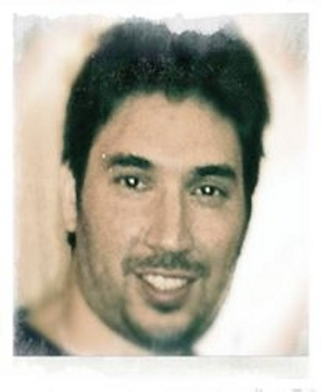
\includegraphics[width=0.6\columnwidth]{photo}
	\vspace{-7cm}
\end{figure}

\begin{flushright}\small
	Dario Palminio \\
	\url{dario.palminio@gmail.com}  \\
	\url{www.palminio.com.ar} \\
	(000) 000-0000
\end{flushright}\normalsize
\framebreak


% Right frame
%%%%%%%%%%%%%%%%%%%%
\Huge\bfseries {\color{RoyalBlue} Dario Palminio} \\
\Large\bfseries  Systems Engineer \\

\normalsize\normalfont

% About me
\begin{AboutMe}
(Incomplete) Add text here.
\end{AboutMe}

% Education
\CVSection{Education}
\CVItem{2010 - present, Lorem ipsum dolor}\\
(Incomplete) Add text here.
\SmallSep

\CVItem{2007 - 2010, Lorem ipsum dolor}\\
(Incomplete) Add text here.
\SmallSep

\CVItem{2005 - 2007, Vivamus vel bibendum}\\
(Incomplete) Add text here.
\Sep

% Experience
\CVSection{Experience}
\CVItem{May 2010 - present, Lorem ipsum}\\
(Incomplete) Add text here.
\SmallSep

\CVItem{Aug 2007 - Feb 2010, Vivamus vel}\\
(Incomplete) Add text here.
\Sep

% Skills
\CVSection{Skills}
\CVItem{Platforms}
\begin{multicols}{3}
\begin{compactitem}[\color{RoyalBlue}$\circ$]
	\item Lorem 
	\item Ipsum 
\end{compactitem}
\end{multicols}
\SmallSep

\CVItem{Computer software}
\begin{multicols}{3}
\begin{compactitem}[\color{RoyalBlue}$\circ$]
	\item Lorem 
	\item Ipsum 
	\item Dolor 
	\item Sit 
	\item Amet
	\item Consectetur 
	\item Adipiscing 
	\item Elit
	\item \ldots
\end{compactitem}
\end{multicols}
\Sep 

\CVSection{Something other}
(Incomplete) Add text here.

\clearpage
\framebreak
\framebreak

\CVSection{Something else}
(Incomplete) Add text here.
\Sep

% References
\CVSection{References}
(Incomplete) Add text here.

%%%%%%%%%%%%%%%%%%%%%%%%%%%%%%%%%%%%%
% End document
%%%%%%%%%%%%%%%%%%%%%%%%%%%%%%%%%%%%%
\end{document}
